\documentclass[border=0pt]{standalone}
\usepackage{tikz}
\usetikzlibrary{positioning,shapes,arrows.meta,patterns,calc}
\definecolor{garnet}{HTML}{73000A}
\definecolor{coral}{HTML}{CC2E40}
\definecolor{slate}{HTML}{466A9F}
\definecolor{teal}{HTML}{1F414D}
\definecolor{olive}{HTML}{65780B}
\definecolor{lime}{HTML}{CED318}
\definecolor{gold}{HTML}{A49137}
\begin{document}
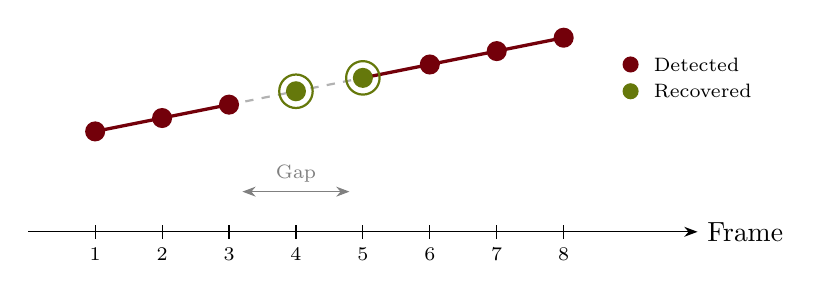
\begin{tikzpicture}[scale=0.85]
    % Time axis
    \draw[-{Stealth}, black] (0,0) -- (10,0) node[right] {Frame};
    \foreach \x/\label in {1/1, 2/2, 3/3, 4/4, 5/5, 6/6, 7/7, 8/8} {
        \draw[black] (\x,0.1) -- (\x,-0.1) node[below, font=\scriptsize] {\label};
    }
    
    % Track line
    \draw[garnet, very thick] (1,1.5) -- (2,1.7) -- (3,1.9);
    \draw[gray!60, thick, dashed] (3,1.9) -- (4,2.1) -- (5,2.3);
    \draw[garnet, very thick] (5,2.3) -- (6,2.5) -- (7,2.7) -- (8,2.9);
    
    % Points
    \foreach \x/\y in {1/1.5, 2/1.7, 3/1.9, 6/2.5, 7/2.7, 8/2.9} {
        \fill[garnet] (\x,\y) circle (0.15);
    }
    
    % Recovered points
    \foreach \x/\y in {4/2.1, 5/2.3} {
        \fill[olive] (\x,\y) circle (0.15);
        \draw[olive, thick] (\x,\y) circle (0.25);
    }
    
    % Gap annotation
    \draw[{Stealth}-{Stealth}, gray] (3.2,0.6) -- (4.8,0.6);
    \node[above, font=\scriptsize, gray] at (4,0.6) {Gap};
    
    % Legend
    \fill[garnet] (9,2.5) circle (0.12);
    \node[right, font=\scriptsize] at (9.2,2.5) {Detected};
    \fill[olive] (9,2.1) circle (0.12);
    \node[right, font=\scriptsize] at (9.2,2.1) {Recovered};
\end{tikzpicture}
\end{document}
